\section{Results}
\label{sec:results}
This section describes the experimental results of the final recognition system. It includes the performance of the individual steps: painting segmentation, the matching algorithm and room localization. 


\subsection{Dataset}
The main dataset consists of 688 pictures of all art items in the museum which functions as a database. These pictures are taken at eye-level height and each picture contains one or multiple art items. One part of the dataset is taken with a Nokia 7 Plus camera, which offers a base resolution of 3024 by 4032 pixels and the other part is taken with a Samsung A3 2016, which offers a base resolution of 3096 by 4128 pixels. All pictures in the dataset are compressed to 1000 x 1000 pixels. To reduce the load time of this dataset, a prebuilding stage was implemented. This stage reduces each image to a collection of interest points and corresponding descriptors for these interest points as generated by the ORB \cite{Rublee2011} algorithm. 

\subsection{Test set}
Apart from the dataset, two different testing sets exist to evaluate the algorithm. The first testing contains still images of various shots at the museum. This dataset contains more difficult examples such as steep angles or hard to detect paintings. A random sample ($n = 30$) was selected and labeled manually. This first test set is used to evaluate the segmentation and matching part. A second testing set are various videos which emulates a person recording paintings while moving trough the museum. Similar to the first test set, a small segment (1 minute) of the video was taken and labeled manually. This last test set is used to evaluate path tracking. An advantage of the test set is that these are still images and as such, are unlikely to be subjected to motion blur, which increases the difficulty of segmentation and matching.

\subsection{Segmentation Accuracy}
The random sample from the test set was first manually segmented to indicate a perfect segmentation. This results in 4 coordinates of a polygon which represent the ideal polygon. Afterwards, the segmentation is done automatically by the algorithm, which also gives four coordinates of a polygon. To illustrate, both polygons are shown on figure \ref{fig:painting_segmentation_validation_1}.
To measure the similarity of these two polygons, and thus the correctness of the segmentation, we first calculate the intersection area $A_i$ and the area of the ideal polygon $A_{pi}$. The ratio of $A_i$ to $A_{pi}$ describes the closeness of two polygons with 100\% being a perfect match and 0\% meaning there is no intersection at all between the two polygons. There is one case where this statistic does not work. When the ideal polygon is fully enclosed by the predicted polygon, $A_i$ will be equal to $A_{pi}$, resulting in a fake perfect match. To prevent this, the roles of the green and red polygon are switched such that we now consider the area of the predicted polygon, $A_{pp}$, instead of $A_{pi}$.

Using this metric, the segmentation method achieves 88.57\% correctness score. Due to the use of the Canny edge detector, the segmentation works fairly well when the painting frame and the background wall differ greatly in color intensity. Problems start to arise when shadows are visible (figure \ref{fig:negative_case_shadow}) or when the painting frame is not fully visible. In the former case, the shadow and the background wall also differ in color intensity, resulting in an edge. These edges usually extend the painting frames and because the contour with the largest area is sought after, the segmentation step will include the shadow as part of the painting.


\begin{figure}
	\centering
	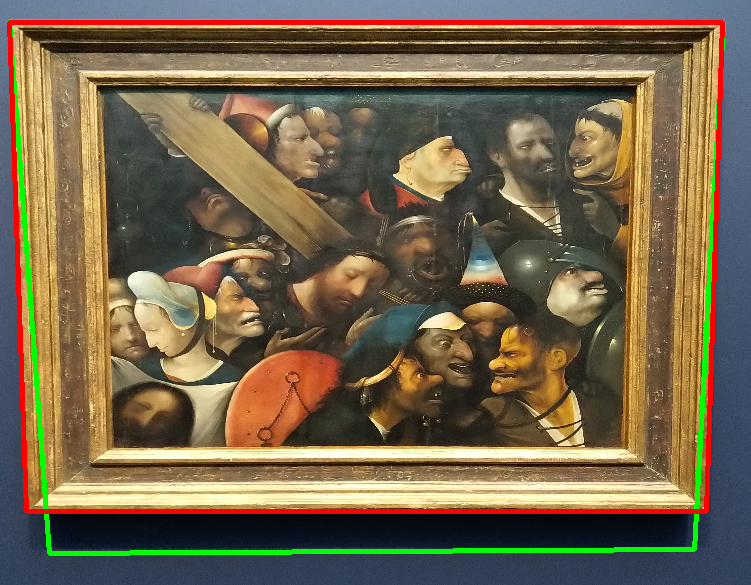
\includegraphics[width=\linewidth]{painting_segmentation_validation_1}
	\caption{A comparison of a manually selected polygon (red) and the polygon found by the segmentation algorithm (green).}
	\label{fig:painting_segmentation_validation_1}
\end{figure}
\begin{figure}
	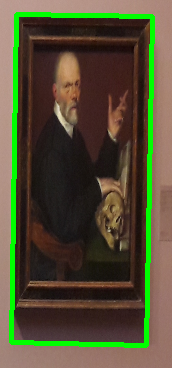
\includegraphics[width=0.5\linewidth]{negative_case_shadow}
	\caption{An example of a shadow underneath the painting. This usually results in the segmentation algorithm to include this shadow as part of the painting because of the strong edge.}
	\label{fig:negative_case_shadow}
\end{figure}


\subsection{Matching Accuracy}
The matching algorithm has to be evaluated manually by comparing the matcher's result. The correctness of the matching algorithm is simply the ratio of the correct matches against the false matches.

To evaluate the room localization, a sample of the video dataset was taken. The generated path is compared against the actual path.

Because our method relies heavily on edge detection, there are cases where this could have a negative impact. In many cases, there is a shadow underneath the painting, as shown on figure \ref{fig:negative_case_shadow}.



\subsection{Qualitative analysis}
In this subsection, we will present a qualitative analysis of our algorithm. We will discuss its strengths, flaws and, with each point, present an example case to help as a visual aid. The flaws in particular help paint a picture of what can be done better in a future iteration of the algorithm. 


One of the algorithm's major strengths lies in its simplicity. The block diagram shows a very linear approach to the problem with concrete begin- and endpoints. Though machine learning is often used in the field of computer vision and has a lot of benefits, the algorithm does not employ it. We do not deny its usefulness and believe that it may be beneficial to implement it in a future version of the algorithm. The classification of pixels may be one of the problems tackled as a way of assisting the segmentation. Even though the algorithm's simplicity is presented as one of its strengths, it can also be considered as one of its weaknesses, much like a double-edged sword.


Furthermore, the algorithm works relatively fast for matching and determining the location of a potential user using a single image. When taking the average of 30 runs of the algorithm with a frame, we get a time of $0.78\pm0.01 s$. Even though this is nearing almost a second, it is important to note that it is expected to take some time to complete as the dataset being matched against is quite large. This will be discussed more in depth further below.


In addition, the use of ORB causes the results of each program run to be invariant given the same input image, implying a deterministic nature. This is of course on the premise that certain parameters such as the Canny thresholds remain the same between runs. Figure \ref{fig:double} shows how two images have the same match and detected keypoints between two runs. However, due to not detecting different potential candidate matches between runs results in the algorithm never being able to present a different solution for the given image.


On top of that, the algorithm is resilient when it can not successfully segment an image. The default behavior is trying to find a frame, extract it, and using it as the input of the matching stage of the algorithm. If no frame can be found, rather than ignoring the current video frame or image, we supply the entire thing to be matched. This may slow the matching stage down by a small margin but has the benefit of still being able to spit out a potential positive match. Figure \ref{fig:full_frame} shows an example where an entire frame is supplied to the matching function, but still manages to find a correct match. This resiliency comes at a price. The matching phase performs slightly worse, as the frame may contain additional features that can help with matching a painting. Should this algorithm be used in an actual application, this can occur when the user is standing too close to a painting. 


As was hinted in the previous point, supplying a full frame or image to the matching phase may slow things down. The input image's size definitely affects the time needed to complete in a negative way. Therefore, images used for the segmentation and matching phases are resized to between \verb|25%-50%| their original size. This may result in some loss of precision but should not affect the overall efficiency of the algorithm. Table \ref{tab:quadratic} shows that resizing an image from the query set to a quarter of its size quadratically decreases the amount of pixels needed to evaluate. The same resizing is applied to the building stage of the database.

\begin{table}[]
	\centering
	\begin{tabular}{rcccl}
		\multicolumn{1}{l}{} & \textbf{Width} & \textbf{Height} & \textbf{Total pixels} &  \\
		\textbf{Original}    & 2322           & 4128            & 9 585 216             &  \\
		\textbf{Resized}     & 580.5          & 1032            & 599 076               & 
	\end{tabular}
	\caption{Taking a 9.5 megapixel picture and resizing it to a quarter of its original size results in a decrease of total pixels by a factor of 16}
	\label{tab:quadratic}
\end{table}

Another problem arises due to an assumption in the matching stage. A match is determined by the smallest sum of distances calculated over the matches between two images. This assumption works well when the amount of matches is fixed between every match between the query image and the training set. ORB detects keypoints and associates descriptors up to a maximum of 200. But what if it can not detect a lot of keypoints, maybe even none? Figure \ref{fig:flat_surface} shows how paintings that have a relative 'flat' surface without discerning features (sometimes even to the naked eye) have trouble being matched to a picture in the data set. Suppose that the segmentation phase detects such a painting and supplies it to the matching phase. A cascade of erroneous matches and room localizations may occur. The inverse is also true, as having an entry in the data set with few keypoints can result in a painting with many keypoints being wrongfully matched with a 'flat' one.


Figure \ref{fig:smaller_rectangle} shows the flaws of the segmentation phase. If no quad can be approximated from the painting then there is a chance that polygons with a smaller surface area may be erroneously detected and fed to the matching stage. The problem lies in the combination of using the Canny operator along with the approximation of quad polygons. Our algorithm is unable to deal with 'valid' paintings that have an approximated polygon with an amount of sides higher than 4.


The final major flaw that will be presented lies in the matching phase: matching a painting is done by doing a linear lookup in the database. For a single image this does not pose that much of a problem. The same can not be said when we expanded our algorithm to analyze the frames of a video. This slowdown is mitigated through two changes to the original algorithm. First, we run it only every 30 or so video frames which is equivalent to around 1 second in real life. Suppose the user is using their smart phone's camera, even when running, it will take some time to cross from one room to the other. Finally, the algorithm offloads the matching procedure to a multi-threading environment, freeing the video code from freezing. But what causes this in the first place? 


Considering there are 688 pictures in the database, coupled with the keypoints and descriptors that were extracted during the prebuilding phase, are matched with the descriptors of the segmented painting results in a total. In our solution, we limit the amount of keypoints and descriptors by 200, which still results in 27 520 000 elements needing to be compared to during each matching phase. Another problem lies in the use of the brute force matching, which tries to compare the keypoints and descriptors of the segmented painting with this dataset. Our original design of this algorithm anticipated that a linear lookup would not pose a problem for our assumed small database of 688 paintings. Szeliski (2010) \todo{ref + add} suggests that a linear lookup has $O(n^{2})$ behavior as the database starts to grow. Our algorithm seems to prove this suggestion. A future iteration of this algorithm may need to place the focus on this part of the algorithm.


\begin{figure}
	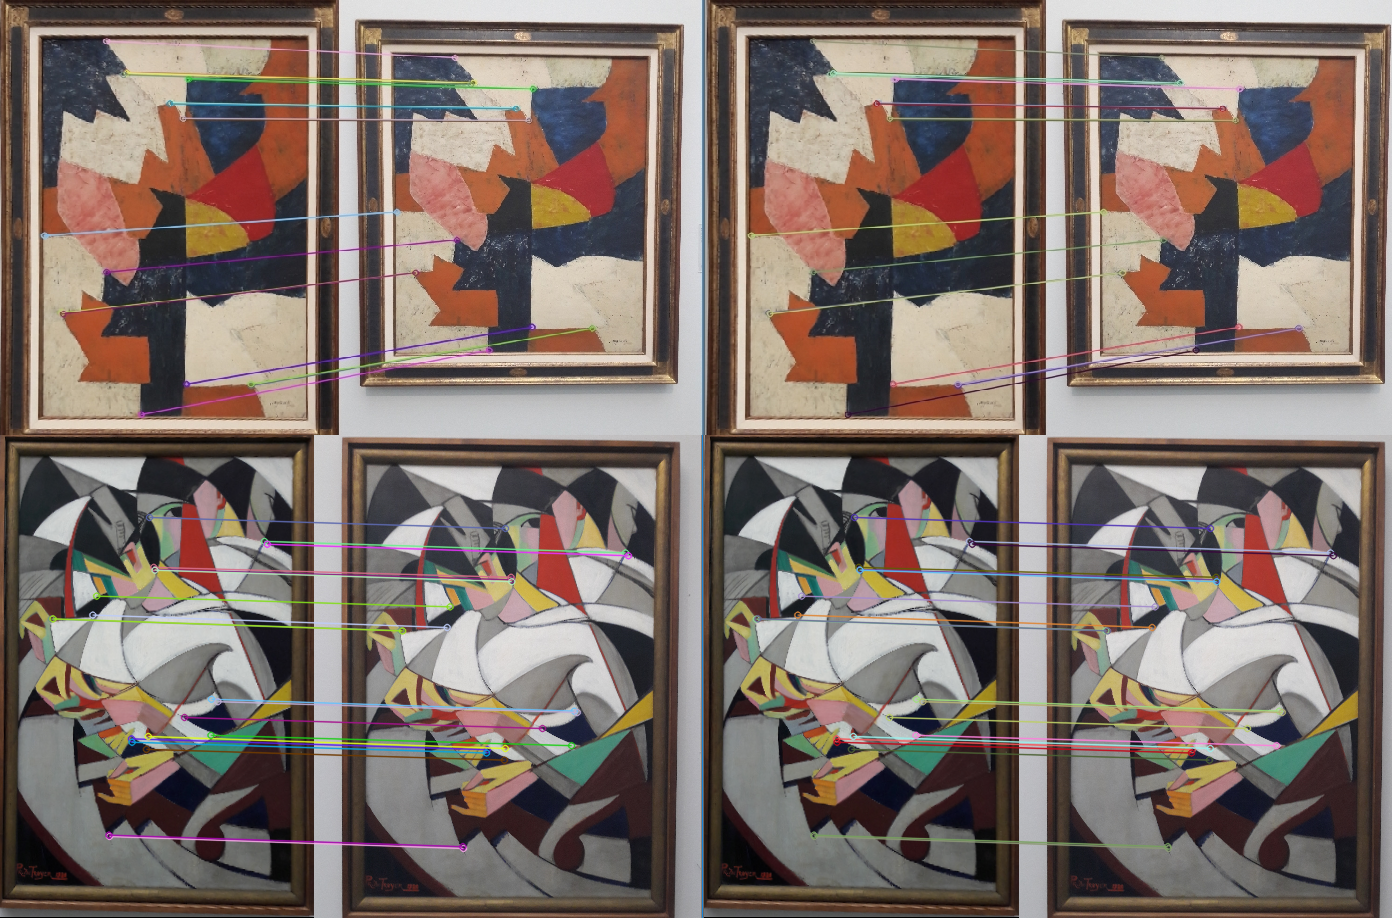
\includegraphics[width=\linewidth]{double}
	\caption{Two different extracted paintings being matched with the database show that with the same Canny thresholds the same match will be returned}
	\label{fig:double}
\end{figure}

\begin{figure}
	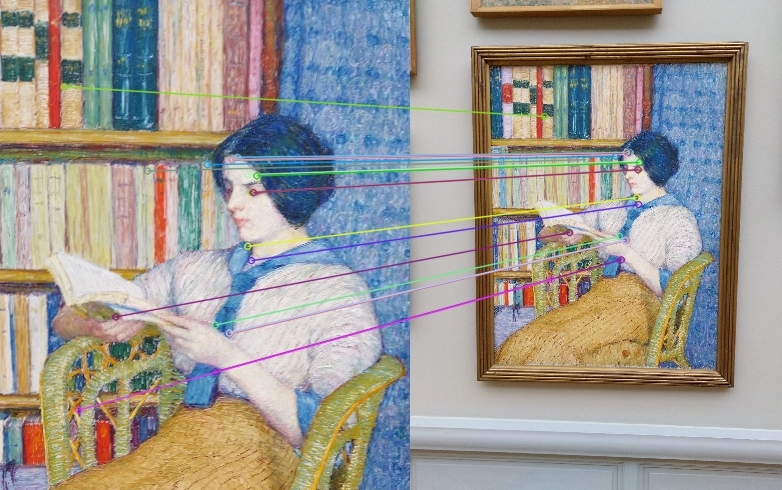
\includegraphics[width=\linewidth]{full_frame}
	\caption{Matching of an entire frame or a closeup of a painting may still yield a correct match}
	\label{fig:full_frame}
\end{figure}

\begin{figure}
	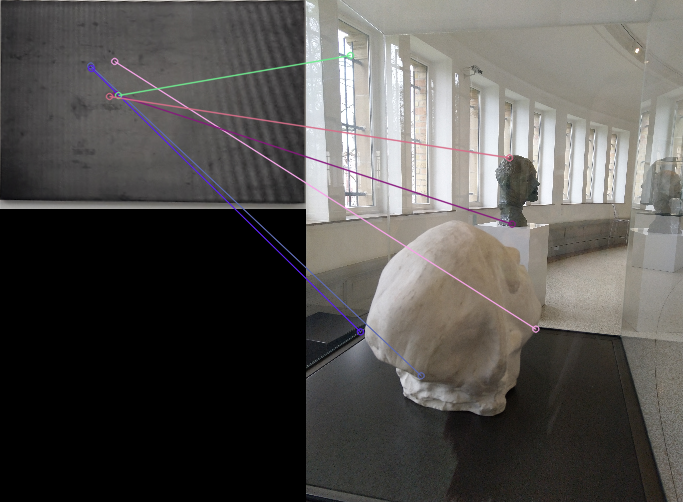
\includegraphics[width=\linewidth]{flat_surface}
	\caption{The extracted painting from the frame is grayish and looks 'flat'. There are not many keypoints that can be detected and successfully matched in this case resulting in a false overall match.}
	\label{fig:flat_surface}
\end{figure}

\begin{figure}
	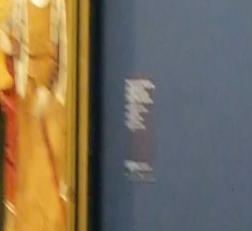
\includegraphics[width=\linewidth]{smaller_rectangle}
	\caption{Information about the paintings hanging next to them have a polygonal shape and may be extracted erroneously}
	\label{fig:smaller_rectangle}
\end{figure}